\begin{atiTask}[
	title = Eine Zombieapokalypse,
	language = Deutsch
]
	Auf einer kleinen Insel gerät ein Virus in Umlauf, der die Bevölkerung in Zombies verwandelt.
	Jeder Infizierte hat in einer Zeitspanne $\tau\in\setReal^+$ Kontakt mit $\tau\cdot k$ anderen Personen, die teilweise ebenfalls infiziert, teilweise aber auch gesunde Menschen sind, wobei $k\in\setReal^+$ gilt.
	Gerät ein gesunder Mensch in Kontakt mit einem Zombie, so wird dieser infiziert.
	\medskip
	\begin{atiSubtasks}
		\item{\locallabel{a}
			Stellen Sie eine Differentialgleichung auf, die dieser Zombieapokalypse genügt.
			Verwenden Sie $N\in\setNatural$ für die Größe der Inselbevölkerung, $Z(t)\in[0,N]$ für die Anzahl der Infizierten, $M(t)\in[0,N]$ für die Anzahl der Gesunden und $t\in\setReal^+$ als freien Parameter der Zeit.

			\begin{atiNote}
				Betrachten Sie zunächst nur die Infizierten zum Zeitpunkt $t+\tau$ und überführen Sie die Differenzengleichung durch Grenzwertbildung in die gesuchte Differentialgleichung.
			\end{atiNote}
		}
		\item{\locallabel{b}
			Lösen Sie diese Differentialgleichung und das folgende Anfangswertproblem.
			\[
				t_0\define 0\separate Z_0\define Z(0) \define \frac{N}{21}
			\]
		}
		\item{\locallabel{c}
			Skizzieren Sie $Z(t)$ und $M(t)$ für $k=2$, $N=1050$ und $t\in\setReal^+$.
		}
		\item{\locallabel{d}
			\textbf{Zusatz:} Ab wann ist nur noch weniger als $1\appendUnit{\%}$ der Bevölkerung nicht infiziert?
			Wie beeinflussen die Parameter $k$ und $N$ diesen Zeitpunkt?
		}
	\end{atiSubtasks}
\end{atiTask}
\begin{atiSolution}
	\begin{atiSubtaskSolutions}
		\item[\localref{a}]{
			Wir definieren als Erstes den Anteil der gesunden Menschen $\alpha(t)\in[0,1]$ und den Anteil der infizierten Menschen $\beta(t)\in[0,1]$ für alle $t\in\setReal^+$.
			\[
				\alpha(t)\define \frac{M(t)}{N}\separate\beta(t)\define\frac{Z(t)}{N}
			\]
			Wir wählen nun eine festen Zeitpunkt $t\in\setReal^+$.
			Nähern wir für kleine Zeitspannen $\tau\in\setReal^+$ die Anzahl der Personen, die ein Zombie trifft, durch $\tau k$ an, so teilen sich Infizierte und Gesunde entsprechend ihrer Anteile auf diese Anzahl auf.
			% Trifft eine infizierte Person für kleine $\tau\in\setReal^+$ nun $\tau k$ andere Personen, so teilen sich Infizierte und Gesunde entsprechend ihrer Anteile $\alpha(t)$ und $\beta(t)$ auf diese Anzahl auf.
			\[
				\tau k \approx \tau k\alpha(t) + \tau k\beta(t)
			\]
			Die Anzahl $S(t)$ der gesunden Menschen, die ein Zombie in der Zeitspanne $\tau$ trifft und infiziert, kann demnach wie folgt für kleine $\tau$ approximiert werden.
			\[
				S(t) \approx \tau k \alpha(t) = \frac{\tau k}{N} M(t)
			\]
			Diese Approximation gilt für jeden Zombie.
			Dementsprechend lässt sich nun die Anzahl der Zombies $Z(t+\tau)$ nach der Zeitspanne $\tau$ beschreiben.
			% Damit ergibt sich die Gesamtanzahl $\Delta Z(t)$ der gesunden Menschen, die während dieser Zeitspanne $\tau$ infiziert werden, durch eine Multiplikation von $S(t)$ mit der Anzahl aller Zombies $Z(t)$.
			% \[
			% 	\Delta Z(t) = S(t)Z(t) = \tau k\alpha(t)Z(t) = \frac{\tau k}{N}M(t)Z(t) = \frac{\tau k}{N} \boxBrackets{N-Z(t)}Z(t)
			% \]
			\[
				Z(t+\tau) \approx Z(t) + S(t)Z(t) = Z(t) + \frac{\tau k}{N} \boxBrackets{N-Z(t)}Z(t)\atiPoints[1]
			\]
			\[
				\implies \frac{Z(t+\tau)-Z(t)}{\tau} \approx \frac{k}{N}\boxBrackets{N-Z(t)}Z(t)
			\]
			Um die Fehler der Näherung mithilfe einer Differentialgleichung zu korrigieren, bildet man den Grenzwert der erhaltenen Differenzengleichung für $\tau\converges 0$.
			\[
				Z'(t) = \lim_{\tau\converges 0}\frac{Z(t+\tau)-Z(t)}{\tau} = \frac{k}{N}\boxBrackets{N-Z(t)}Z(t)
			\]
			\[
				\implies Z' = \frac{k}{N}(N-Z)Z \atiPoints[1]
			\]
		}
		\item[\localref{b}]{
			Bei der oben beschriebenen Gleichung handelt es sich offensichtlich um eine separable Differentialgleichung.
			Die Methode der Trennung der Variablen ergibt dann das Folgende.
			\[
				\frac{Z'(t)}{\boxBrackets{N-Z(t)}Z(t)} = \frac{k}{N} \implies \integral{t_0}{t}{\frac{Z'(s)}{\boxBrackets{N-Z(s)}Z(s)}}{s} = \integral{t_0}{t}{\frac{k}{N}}{s}
			\]
			\[
				\implies \integral{Z_0}{Z(t)}{\frac{1}{(N-s)s}}{s} = \frac{k}{N}(t-t_0)\atiPoints[1]
			\]
			Für die Lösung des Integrals zeigt sich eine Partialbruchzerlegung als sinnvoll.
			\[
				\frac{1}{(N-s)s} = \frac{N}{N}\frac{1}{(N-s)s} = \frac{1}{N}\frac{N-s+s}{(N-s)s} = \frac{1}{Ns} - \frac{1}{N(s-N)}
			\]
			\[
				\implies \integral{Z_0}{Z(t)}{\frac{1}{(N-s)s}}{s} = \integral{Z_0}{Z(t)}{\frac{1}{Ns}}{s} - \integral{Z_0}{Z(t)}{\frac{1}{N(s-N)}}{s}
			\]
			\[
				= \frac{1}{N}\ln\boxBrackets{\frac{Z(t)}{Z_0}} - \frac{1}{N}\ln\boxBrackets{\frac{Z(t)-N}{Z_0-N}} = \frac{1}{N}\ln\roundBrackets{\frac{Z(t)\boxBrackets{Z_0-N}}{Z_0\boxBrackets{Z(t)-N}}}\atiPoints[+1]
			\]
			Die Lösung des Integrals wird nun eingesetzt und die entstehende Gleichung wird explizit nach $Z(t)$ umgestellt.
			\[
				\frac{Z(t)}{Z(t)-N} = \frac{Z_0e^{k(t-t_0)}}{Z_0-N} = -Ae^{k(t-t_0)}\separate A\define \frac{Z_0}{N-Z_0}
			\]
			\[
				\implies Z(t) = \frac{NAe^{k(t-t_0)}}{1 + Ae^{k(t-t_0)}} = N\roundBrackets{1 - \frac{1}{1+Ae^{k(t-t_0)}}}\atiPoints[1]
			\]
			Nun setzen wir die Anfangswerte ein und unterstreichen unser Ergebnis doppelt.
			\[
				A = \frac{1}{20} \implies Z(t) = N\roundBrackets{1 - \frac{1}{1+\frac{1}{20}e^{kt}}}\atiPoints[1]
			\]
		}
		\item[\localref{c}]{
			Die nachfolgende Skizze zeigt die Werte $M(t)$ und $Z(t)$ für verschiedene Zeiten $t\in\setReal^+$.
		}
		\item[\localref{d}]{
			Es sei $\alpha^*\in\roundBrackets{0,1-\frac{Z_0}{N}}$ eine feste Grenze für den Anteil der Menschen.
			Wir suchen nun den frühesten Zeitpunkt $t^*\in\setReal^+$, sodass $\alpha(t^*)\leq\alpha^*$ gilt.
			Durch Äquivalenzumformungen zeigt man, dass $t^*$ existiert und eindeutig ist.
			\[
				\alpha^* = \alpha(t^*) = 1-\beta(t^*) = 1 - \frac{Z(t^*)}{N} = \frac{1}{1 + Ae^{k(t^*-t_0)}}
			\]
			\[
				\implies t^* = t_0 + \frac{1}{k}\ln\boxBrackets{\frac{1}{A}\roundBrackets{\frac{1}{\alpha^*}-1}} = t_0 + \frac{1}{k}\ln\boxBrackets{\frac{N-Z_0}{Z_0}\roundBrackets{\frac{1}{\alpha^*}-1}}
			\]
			Setzt man nun die gewünschten Werte der Parameter ein, so erhält man das folgende Ergebnis.
			\[
				t_0 = 0\separate k=2\separate A = 0.05 \separate\alpha^* = 1\appendUnit{\%}\implies t^* = \frac{\ln 1980}{2} \approx 3.8\atiPoints[+1]
			\]
			Zu beachten ist, dass $t^*$ sowohl von $k$ als auch von $N$ abhängig ist.
			Steigt $k$, so verringert sich $t^*$.
			Steigt $N$, so erhöht sich auch $t^*$.\atiPoints[+1]
		}
	\end{atiSubtaskSolutions}
	\begin{figure}[H]
		\center
		\atiPoints[2]
		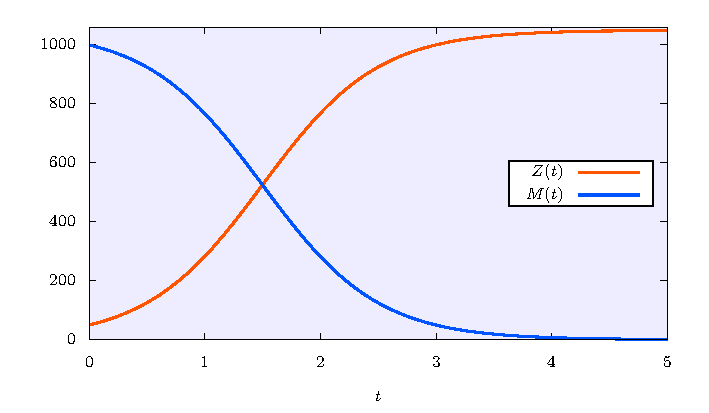
\includegraphics[width=0.9\textwidth]{task-eine_zombieapokalypse-diagram}
		\caption{Die Abbildung zeigt die Anzahl der Zombies $Z(t)$ und der gesunden Menschen $M(t)$ für verschiedene Zeiten $t$.}
	\end{figure}
\end{atiSolution}